\chapter{Спин, измерение и двумерное пространство состояний}

\lectureoverview{Спин имеет направление, однако каждое измерение одной из его компонент даёт только \(+1\) или \(-1\). Сначала мы сформулируем эту операционную проблему, а затем увидим, почему обычная логика множеств не работает для несовместимых измерений. Подходящий язык даёт двумерное комплексное векторное пространство: вероятности возникают из амплитуд, различимые альтернативы ортогональны, а базисы вверх--вниз, вправо--влево и внутрь--наружу кодируют три пространственных направления, не превращая вектор состояния в обычную стрелку.}

\section{От кубита к спину}

Система с двумя состояниями, введённая как кубит, теперь будет называться \emph{спином}. Эта смена названия вводит в обсуждение пространственное направление, но вместе с тем создаёт опасность, связанную со словом \emph{вектор}. Нужно различать два разных объекта:

\begin{definition}
\emph{Трёхвектор} — это обычный действительный вектор в трёхмерном пространстве. Без уточнения \emph{вектор} будет означать элемент абстрактного векторного пространства, такого как комплексное пространство состояний, используемое в квантовой механике.
\end{definition}

Спин можно приготовить относительно оси в обычном пространстве. Однако его состояние будет представляться абстрактным вектором. Связь между этими двумя утверждениями — одна из тех вещей, которые мы должны выяснить; её нельзя просто принять на основании картинки.

\section{Почему прибор нельзя исключить}

Классическая механика побуждает нас воображать идеального наблюдателя, который узнаёт о системе, возмущая её сколь угодно слабо. Предположим, например, что мы хотим увидеть макроскопический объект. Мы освещаем его, собираем отражённый свет линзой и усиливаем изображение. Свет оказывает некоторую силу, но в классической идеализации его интенсивность можно уменьшать, одновременно увеличивая усиление. Возмущение можно сделать сколь угодно малым, не отказываясь от самой идеи измерения.

В квантовой механике эта предельная процедура не работает. Прибор можно совершенствовать, экранировать и калибровать, но измерение, вообще говоря, нельзя сделать одновременно информативным и сколь угодно мало возмущающим. Что-то в системе изменяется. Это не означает, что каждое измерение уничтожает каждое свойство или что результат нельзя воспроизвести. Это означает, что прибор является частью физического вопроса, который задаётся, и состояние после измерения нельзя игнорировать.

Пока будем рассматривать прибор как чёрный ящик с двумя особенностями: его можно ориентировать в пространстве, а его индикатор регистрирует либо \(+1\), либо \(-1\). Небольшая стрелка на доске служит удобной меткой для приготовленного спина:

\begin{figure}[htbp]
\centering
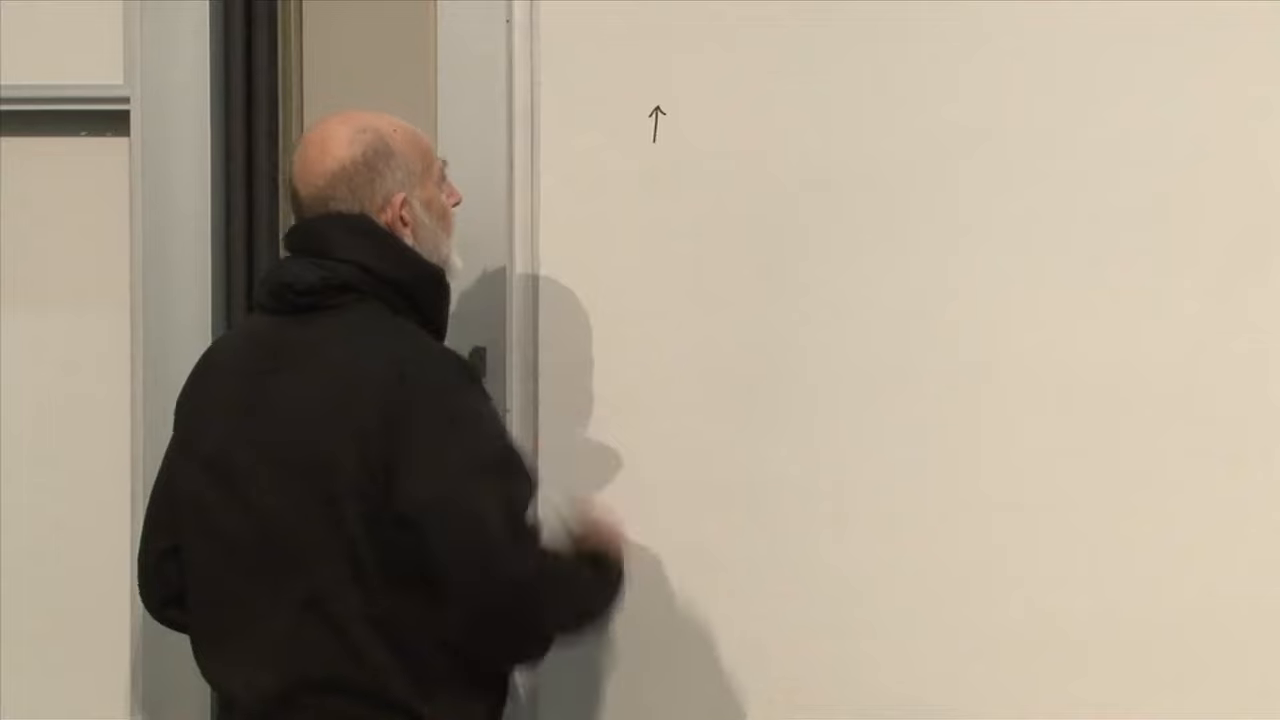
\includegraphics[width=0.64\textwidth]{lecture_02_figure_02.png}
\caption{Первое предварительное обозначение спина, приготовленного вдоль оси. Стрелка обозначает способ приготовления; это ещё не классическая модель состояния.}
\lectureframe{00:05:15}
\end{figure}

Выберем оси так, чтобы \(z\) был направлен вверх по доске, \(x\) — вправо, а \(y\) — из плоскости доски. Если прибор ориентирован вдоль единичного направления \(\hat m\), его результат равен
\begin{equation}
\sigma_{\hat m}=\pm1.
\end{equation}
В частности,
\[
\sigma_z=\pm1,\qquad \sigma_x=\pm1,\qquad \sigma_y=\pm1.
\]
На данном этапе слово \emph{компонента} понимается операционально: \(\sigma_z\) — это то, что показывает ориентированный прибор, когда он направлен вдоль \(z\). Это ещё не \(z\)-компонента скрытой классической стрелки.

\subsection{Повторяемость и возмущение}

Предположим, что измерение \(z\) даёт \(+1\). Если между ними нет никакой промежуточной операции, то второе измерение \(z\) снова даёт \(+1\), как и дальнейшие повторения. Первое измерение подготовило состояние, в котором на тот же вопрос есть определённый ответ.

\begin{classroomqa}
\audiencequestion{Если квантовое измерение возмущает спин, почему при немедленном повторении получается тот же результат?}
\lecturerresponse{Возмущение не является неизбирательным. Измерение \(\sigma_z\) может изменить то, что произошло бы при более позднем измерении по \(x\) или \(y\), оставляя при этом только что измеренное значение \(\sigma_z\) воспроизводимым. Для полезного эксперимента как раз и нужна такая ограниченная форма устойчивости.}
\end{classroomqa}

Теперь поверните прибор на \(180^\circ\). Спин, который при ориентации вверх дал \(+1\), при перевёрнутой ориентации даёт \(-1\). Снова поверните прибор в исходное положение, и результатом будет \(+1\). Следовательно, ориентация существенна. Термометр не показал бы температуру с минусом лишь потому, что его перевернули вверх ногами; анализатор спина ведёт себя иначе, потому что задаёт направленный вопрос.

\begin{figure}[htbp]
\centering
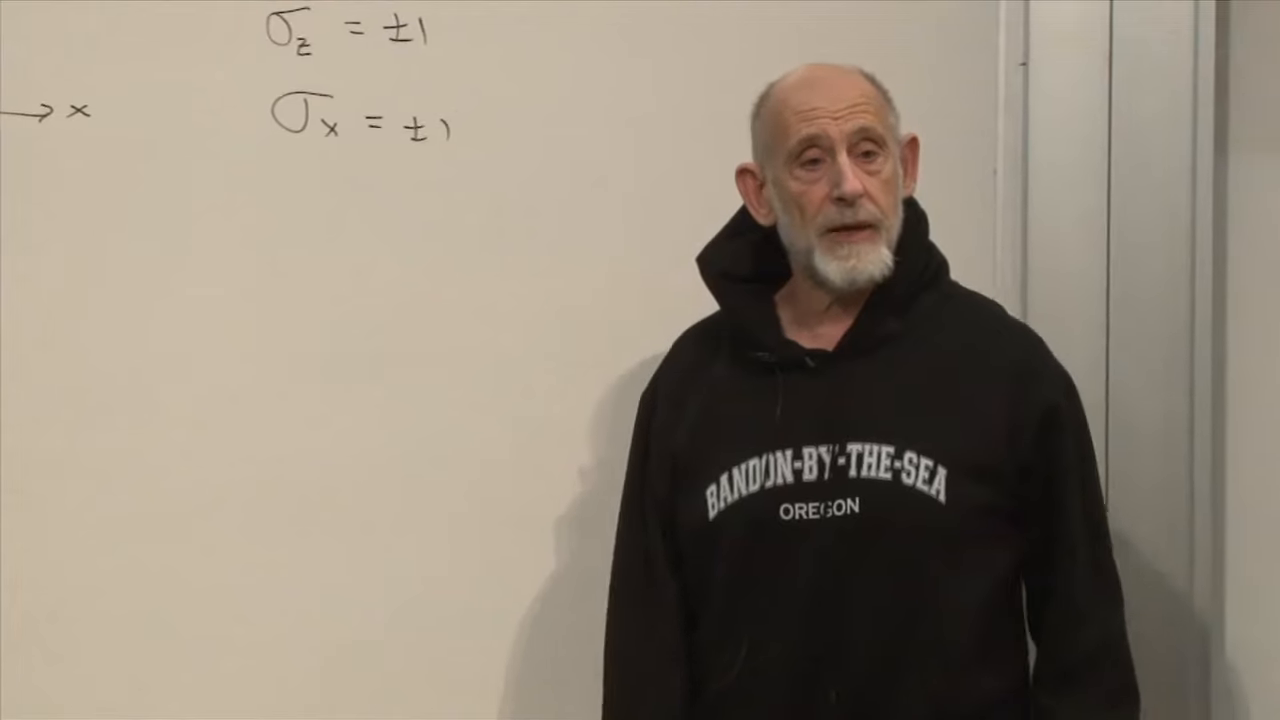
\includegraphics[width=0.72\textwidth]{lecture_02_figure_03.png}
\caption{На доске записаны двузначные метки \(\sigma_z=\pm1\) и \(\sigma_x=\pm1\) вместе с указанием оси \(x\).}
\lectureframe{00:12:46}
\end{figure}

Контраст с классическим единичным вектором виден сразу. Классические компоненты непрерывно меняются между \(-1\) и \(+1\). Единичный вектор, перпендикулярный оси \(x\), имеет нулевую \(x\)-компоненту. Анализатор спина, направленный вдоль \(x\), напротив, никогда не показывает нуль. Он показывает \(+1\) или \(-1\) даже тогда, когда спин был приготовлен вдоль \(z\).

\section{Отдельные результаты и средние, ведущие себя как векторы}

Приготовим спин, получив \(\sigma_z=+1\), а затем измерим \(\sigma_x\). В половине одинаково приготовленных испытаний получается \(+1\), а в половине — \(-1\). Следовательно,
\begin{equation}
\langle \sigma_x\rangle=0.
\end{equation}
Та же подготовка даёт
\begin{equation}
\langle \sigma_y\rangle=0.
\end{equation}
И наоборот, для спина, приготовленного с \(\sigma_x=+1\), вероятности двух исходов последующего измерения по \(z\) или \(y\) равны.

В этом утверждении скрыты два разных эксперимента. Повторное измерение \(\sigma_x\) на \emph{одном и том же} спине после первого результата измерения \(x\) лишь подтверждает этот результат. Чтобы получить статистику пятьдесят--пятьдесят, нужны либо много спинов, приготовленных в одном и том же \(z\)-состоянии, либо один спин, который перед каждым измерением \(x\) снова возвращают к той же подготовке.

\begin{classroomqa}
\audiencequestion{Что происходит, если спин не был специально приготовлен до того, как он попал в прибор?}
\lecturerresponse{Результатом всё равно будет \(+1\) или \(-1\), но вероятности зависят от того состояния, в котором спин фактически находится. Приготовление — это контролируемая процедура, делающая повторные испытания сопоставимыми. Если между двумя измерениями происходит неизвестное воздействие, повторяемость больше не гарантирована; если не происходит ничего, результат для той же компоненты воспроизводим.}
\end{classroomqa}

\subsection{Два произвольных направления}

Приготовьте спин вдоль единичного направления \(\hat n\), получив \(+1\) на анализаторе, ориентированном вдоль \(\hat n\). Затем измерьте вдоль другого единичного направления \(\hat m\). Каждое испытание по-прежнему даёт только \(\pm1\), но среднее по одинаково приготовленным испытаниям равно
\begin{equation}
\boxed{\langle\sigma_{\hat m}\rangle=\hat n\cdot\hat m
=\cos\theta_{nm}.}
\label{eq:spin-average}
\end{equation}
На доске используется более короткая запись \(\langle\sigma_m\rangle=n\cdot m\):

\begin{figure}[htbp]
\centering
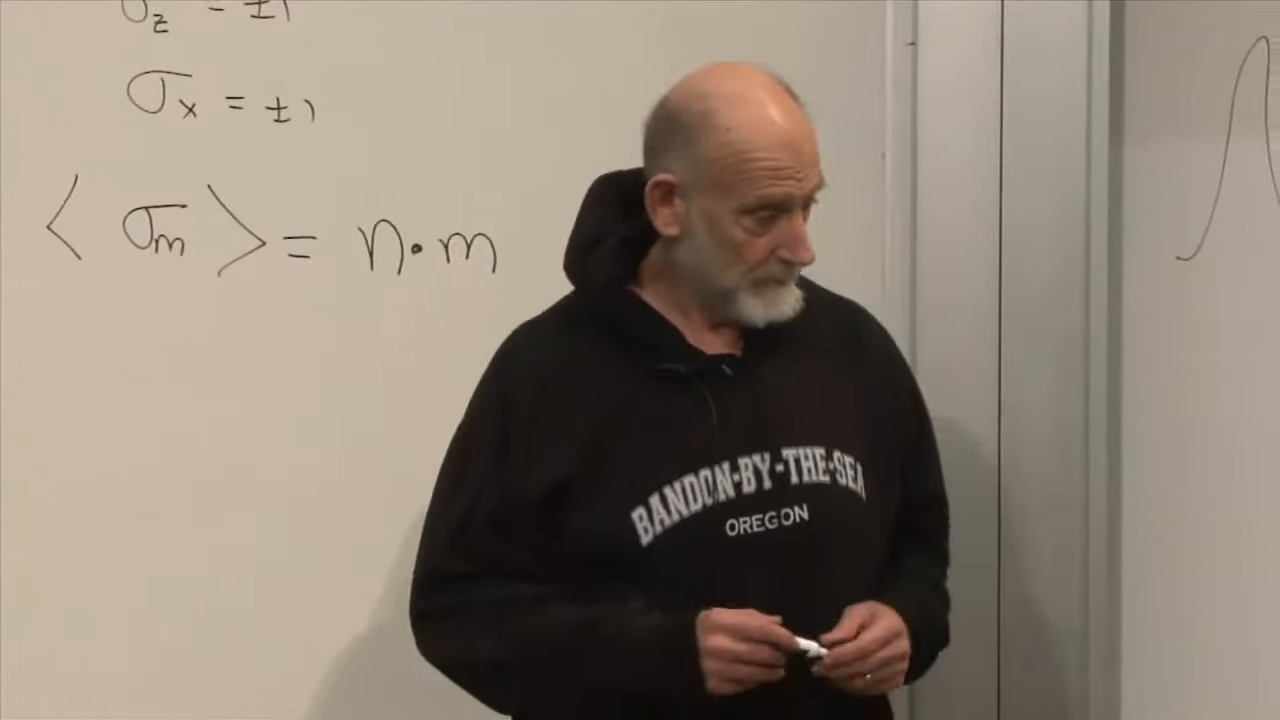
\includegraphics[width=0.74\textwidth]{lecture_02_figure_04.png}
\caption{Вектороподобный закон относится к среднему по ансамблю, а не к отдельному исходу \(\pm1\).}
\lectureframe{00:23:22}
\end{figure}

Уравнение~\eqref{eq:spin-average} охватывает и предыдущие случаи. Если \(\hat m=\hat n\), среднее равно \(+1\); поскольку ни один результат не может превышать \(+1\), каждое испытание даёт \(+1\). Если \(\hat m=-\hat n\), каждое испытание даёт \(-1\). Перпендикулярные оси дают нулевое среднее и равные частоты.

Если \(p_+\) и \(p_-\) обозначают вероятности двух возможных исходов, то
\[
p_++p_-=1,\qquad p_+-p_-=\hat n\cdot\hat m.
\]
Следовательно,
\begin{equation}
p_\pm=\frac{1\pm\hat n\cdot\hat m}{2}.
\label{eq:direction-probabilities}
\end{equation}
\editorialnote{В лекции указаны два исхода и их среднее значение. Уравнение~\eqref{eq:direction-probabilities} является прямым алгебраическим следствием этих двух фактов.}

\begin{classroomqa}
\audiencequestion{Является ли величина в угловых скобках \emph{математическим ожиданием} или обычным средним?}
\lecturerresponse{Это среднее зарегистрированных результатов по многим повторениям. \emph{Математическое ожидание} — стандартный термин, но здесь не имеется в виду никакого дополнительного типа усреднения. Прибор выдаёт список результатов \(+1\) и \(-1\); скобки обозначают среднее арифметическое этого списка в пределе большого ансамбля.}
\end{classroomqa}

\begin{classroomqa}
\audiencequestion{Имела ли стрелка \(\hat n\) уже геометрический смысл до того, как стал известен закон для среднего?}
\lecturerresponse{Сначала это была метка того, как был ориентирован прибор подготовки. Эксперимент с переворачиванием и зависимость среднего от \(\hat n\cdot\hat m\) придают этой метке операциональную геометрию. Прибор определяет, что означают компоненты; отдельный результат никогда не даёт классической проекции.}
\end{classroomqa}

Это первое согласование направленной картины с дискретными данными. Отдельный спин не ведёт себя как классическая стрелка с компонентами, принимающими непрерывные значения. Тем не менее статистика многих одинаково приготовленных спинов преобразуется в точности как компоненты единичного трёхвектора.

\section{Классические высказывания как множества}

Прежде чем строить пространство квантовых состояний, рассмотрим, как работает логика для классической системы. Пусть возможные состояния образуют множество \(\Omega\). Высказывание \(A\) представляется подмножеством состояний, для которых \(A\) истинно.

Для шестигранного кубика
\[
A=\{2,4,6\}
\]
может представлять \emph{результат чётен}, тогда как
\[
B=\{4,5,6\}
\]
может представлять \emph{результат больше трёх}. Логические операции превращаются в операции над множествами:
\begin{equation}
\neg A=A^c,\qquad
A\land B=A\cap B,\qquad
A\lor B=A\cup B.
\label{eq:classical-logic}
\end{equation}
Здесь \(\lor\) — это неисключающее ИЛИ: \(A\lor B\) истинно, когда истинно \(A\), истинно \(B\) или истинны оба. Это не то исключающее повседневное употребление \emph{либо \(A\), либо \(B\), но не оба сразу}.

\begin{classroomqa}
\audiencequestion{У измерения спина есть только два исхода, но направление приготовления меняется непрерывно. Является ли множество состояний конечным или непрерывным?}
\lecturerresponse{Множество возможных направлений приготовления непрерывно, хотя у каждого выбранного анализатора есть только два показания. Именно поэтому одного подсчёта меток детектора недостаточно, чтобы описать пространство состояний.}
\end{classroomqa}

Для классических подмножеств пересечение и объединение не зависят от того, какое высказывание упомянуто первым:
\[
A\cap B=B\cap A,\qquad A\cup B=B\cup A.
\]
Поэтому экспериментальную проверку составного классического высказывания можно идеализировать, не вводя порядок в саму логику.

\section{Проверка ИЛИ, зависящая от порядка}

Рассмотрим квантовые высказывания
\begin{equation}
A:\sigma_z=+1,\qquad B:\sigma_x=+1.
\end{equation}
У каждого высказывания есть ясная проверка. Ориентируйте аппарат вдоль \(z\), чтобы проверить \(A\), или вдоль \(x\), чтобы проверить \(B\). Трудность возникает, когда пытаются проверить \(A\lor B\), сначала проверяя одно высказывание, а если оно ложно, то проверяя другое.

Представьте, что невидимый приготовитель подготовил спин \(z\)-вверх. Если сначала проверяется \(A\), результат заведомо равен \(+1\), и проверка ИЛИ завершается значением \emph{истина}.

Изменим порядок на обратный. Если сначала проверять \(B\), получаем
\[
P(B)=\frac12,\qquad P(\neg B)=\frac12.
\]
Если \(B\) ложно, то измерение \(x\) всё же подготавливает определённое \(x\)-состояние. Проверка \(A\) на этом состоянии даёт
\[
P(A\mid \neg B)=\frac12,\qquad
P(\neg A\mid \neg B)=\frac12.
\]
Следовательно, обратная процедура объявляет оба высказывания ложными с вероятностью
\begin{equation}
P(\neg B\ \text{then}\ \neg A)
=\frac12\cdot\frac12=\frac14.
\end{equation}
Таким образом, при одном порядке ИЛИ принимается всегда, а при другом отвергается в одной четверти испытаний.

\begin{classroomqa}
\audiencequestion{Вызвано ли это противоречие всего лишь нашим неполным знанием о тайно подготовленном состоянии?}
\lecturerresponse{Нет. Скрытую подготовку выбрали только для того, чтобы сделать сравнение более отчётливым. Первое измерение \(x\) физически подготавливает \(x\)-состояние, так что последующая проверка \(z\) выполняется уже на изменённом состоянии. Если наблюдателю дать больше информации об исходной подготовке, это не отменит вмешательства.}
\end{classroomqa}

\begin{classroomqa}
\audiencequestion{Можно ли проверять ИЛИ с помощью более сложной иерархии вопросов, а не по этому последовательному правилу?}
\lecturerresponse{Разумеется, можно определить различные экспериментальные процедуры, но тогда это будут разные квантовые измерения. Не существует независимого от процедуры подмножества \(A\cup B\), истинность которого просто обнаруживается безотносительно к аппарату. Зависимость от порядка служит предупреждением: классическая логика множеств не является собственной логикой этих высказываний.}
\end{classroomqa}

Позже высказывания будут представляться проекционными операторами. Краткое алгебраическое предупреждение таково:
\begin{equation}
P_A P_B\ne P_B P_A.
\end{equation}
Пока больше ничего из теории операторов не требуется. Существенно то, что несовместимые проверки не коммутируют и что их составные высказывания нельзя рассматривать как обычные объединения множеств.

\begin{classroomqa}
\audiencequestion{Можно ли устроить двухчастичную версию этого эксперимента так, чтобы выбор проверки действовал назад во времени?}
\lecturerresponse{Этот вопрос требует аппарата, который здесь ещё не развит. Из последовательности с одним спином не следует никакого вывода об обратной причинности, поэтому вопрос остаётся открытым, вместо того чтобы строить догадки.}
\end{classroomqa}

\section{Линейное пространство состояний}

Множество содержит элементы, но, вообще говоря, нет естественного способа сложить два элемента и получить третий. Линейное векторное пространство обладает большей структурой. Если \(\ket{A}\) и \(\ket{B}\) — векторы, а \(\alpha,\beta\in\mathbb C\), то
\begin{equation}
\alpha\ket{A}+\beta\ket{B}
\end{equation}
есть ещё один вектор в том же пространстве. Квантовые состояния представляются в таком комплексном линейном пространстве.

Каждому кет-вектору \(\ket{A}\) соответствует дуальный бра-вектор \(\bra{A}\). Сопоставление бра с кетом даёт комплексное число, скалярное произведение. Оно обладает сопряжённой симметрией,
\begin{equation}
\braket{A}{B}=\braket{B}{A}^{*}.
\label{eq:conjugate-symmetry}
\end{equation}

\begin{figure}[htbp]
\centering
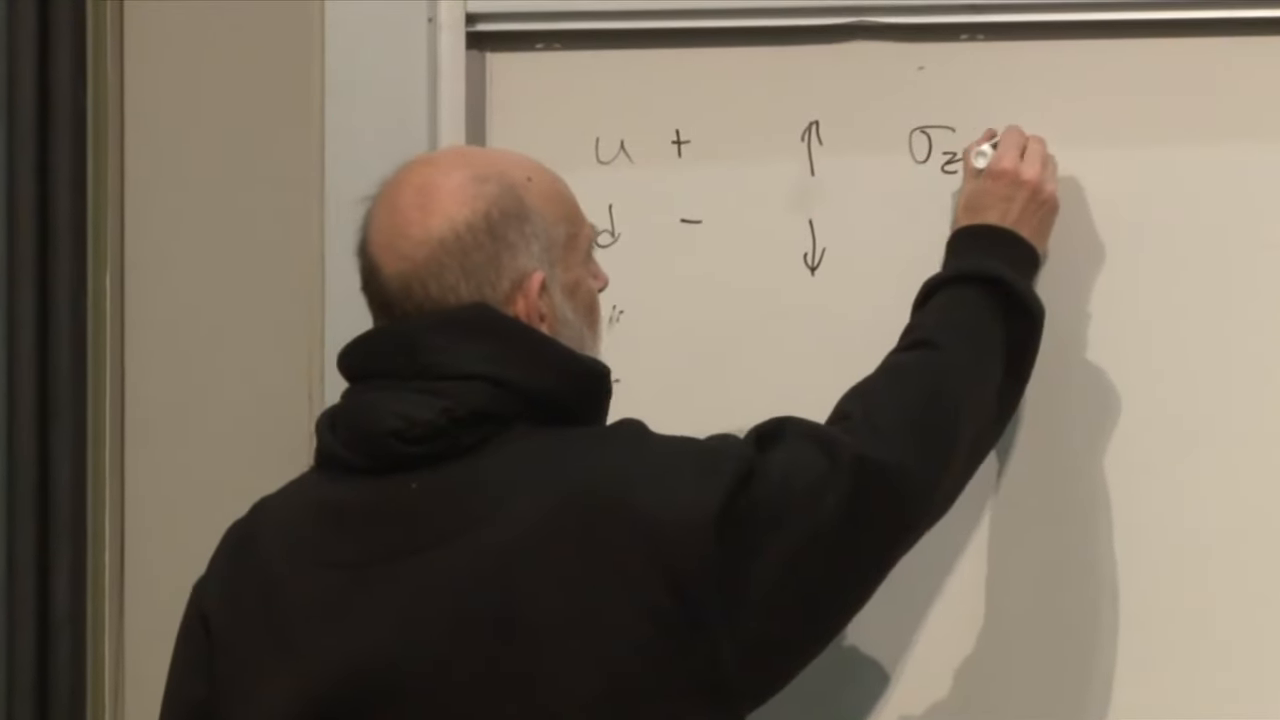
\includegraphics[width=0.78\textwidth]{lecture_02_figure_05.png}
\caption{На доске сведены линейные комбинации и сопряжённая перестановка аргументов скалярного произведения.}
\lectureframe{00:46:53}
\end{figure}

Квадрат длины вектора равен
\begin{equation}
\|\ket{A}\|^2=\braket{A}{A}.
\end{equation}
Из уравнения~\eqref{eq:conjugate-symmetry} следует, что это число равно своему собственному комплексно-сопряжённому и, следовательно, вещественно; аксиомы скалярного произведения также делают его неотрицательным. Два вектора ортогональны, когда
\begin{equation}
\braket{A}{B}=0.
\end{equation}
Размерность пространства — это наибольшее число взаимно ортогональных ненулевых направлений, которые можно выбрать.

\begin{classroomqa}
\audiencequestion{Должен ли каждый базис состоять из взаимно ортогональных векторов?}
\lecturerresponse{Нет. Базису достаточно быть линейно независимым и порождать пространство. Ортогональные базисы особенно удобны, потому что из них легко извлекать коэффициенты и вероятности. В двумерном случае два непараллельных вектора могут образовывать базис, даже когда их скалярное произведение не равно нулю.}
\end{classroomqa}

\section{Двумерное пространство спина}

Постулируется, что пространство состояний одного спина является двумерным комплексным векторным пространством,
\begin{equation}
\mathcal H_{\mathrm{spin}}\cong\mathbb C^2.
\end{equation}
Существует непрерывно много возможных векторов состояния, но для выражения любого из них требуются только два независимых базисных вектора.

Начнём с состояний, подготавливаемых аппаратом, ориентированным вдоль \(z\):
\begin{align}
\ket{u}&\longleftrightarrow \sigma_z=+1,\\
\ket{d}&\longleftrightarrow \sigma_z=-1.
\end{align}
Буквы \(u,d\), знаки \(+,-\) и стрелки \(\uparrow,\downarrow\) — альтернативные обозначения одних и тех же двух подготовок. Поскольку измерение \(z\) различает их с полной определённостью, их векторы состояния ортогональны:
\begin{equation}
\braket{u}{d}=0.
\end{equation}
Выберем их единичной длины,
\[
\braket{u}{u}=\braket{d}{d}=1.
\]

Тогда любое состояние спина можно записать как
\begin{equation}
\ket{A}=\alpha_u\ket{u}+\alpha_d\ket{d},
\qquad \alpha_u,\alpha_d\in\mathbb C.
\label{eq:general-spin-state}
\end{equation}
Правило вероятностей имеет вид
\begin{equation}
P(u|A)=|\alpha_u|^2,\qquad
P(d|A)=|\alpha_d|^2.
\label{eq:born-z}
\end{equation}
Поскольку должен произойти один из двух исходов,
\begin{equation}
|\alpha_u|^2+|\alpha_d|^2=1.
\label{eq:normalization}
\end{equation}

\begin{figure}[htbp]
\centering
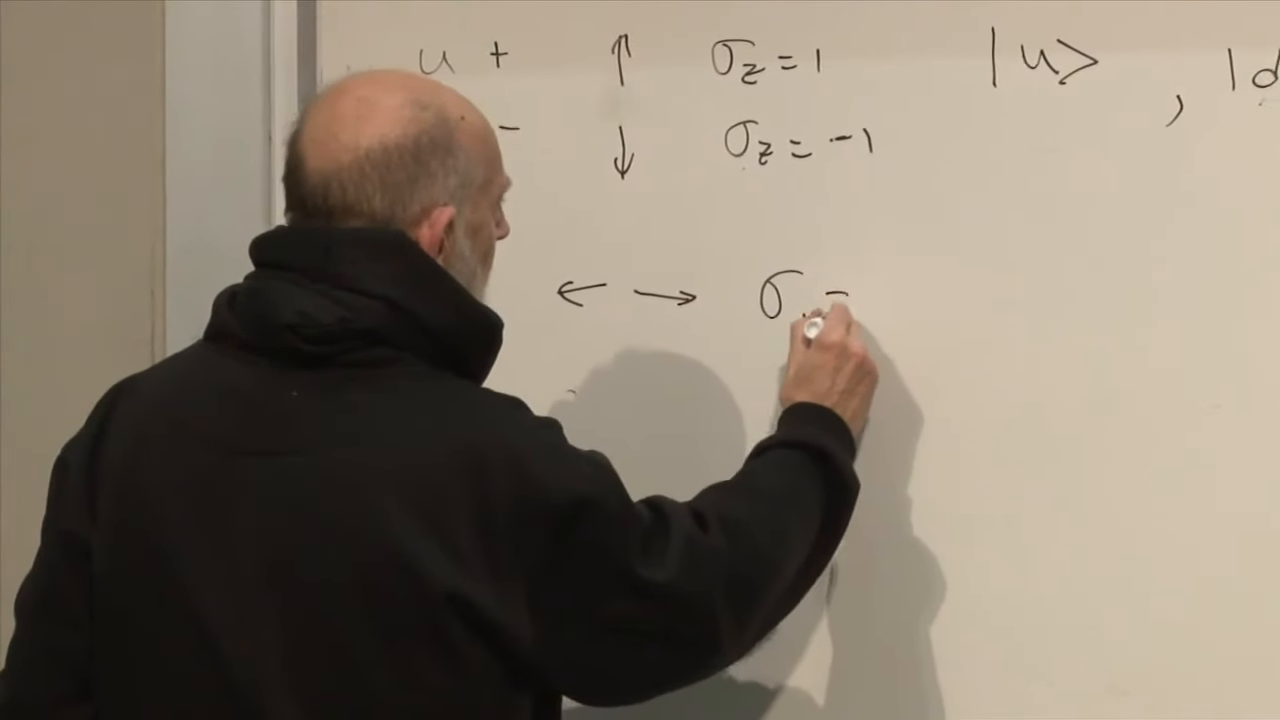
\includegraphics[width=0.78\textwidth]{lecture_02_figure_06.png}
\caption{Общее разложение по состояниям вверх--вниз, сумма вероятностей двух исходов и эквивалентное условие единичной нормы.}
\lectureframe{01:03:38}
\end{figure}

Эквивалентность условию единичной нормировки следует непосредственно:
\begin{align}
\braket{A}{A}
&=(\alpha_u^*\bra{u}+\alpha_d^*\bra{d})
  (\alpha_u\ket{u}+\alpha_d\ket{d})\\
&=|\alpha_u|^2\braket{u}{u}
 +\alpha_u^*\alpha_d\braket{u}{d}\\
&\quad +\alpha_d^*\alpha_u\braket{d}{u}
 +|\alpha_d|^2\braket{d}{d}\\
&=|\alpha_u|^2+|\alpha_d|^2=1.
\end{align}
Итак, физическое чистое состояние представляется нормированным вектором.

\begin{classroomqa}
\audiencequestion{Эти утверждения выводятся или являются постулатами?}
\lecturerresponse{На данном этапе это правила, согласуемые с экспериментами. Двумерное пространство, правило вероятностей и интерпретация ортогональности вводятся эвристически. Их взаимную согласованность уже можно проверить; систематическая связь между состояниями и наблюдаемыми будет рассмотрена дальше.}
\end{classroomqa}

\subsection{Ортогональность как различимость}

Физическое содержание ортогональности полезнее, чем образ перпендикулярных стрелок:

\begin{quote}
Состояния, которые можно с полной определённостью различить одним измерением, представляются ортогональными векторами.
\end{quote}

Состояния вверх и вниз удовлетворяют этому критерию. Если состояние — вверх, аппарат \(z\) никогда не даёт результата вниз, и наоборот. Ненулевое перекрытие означает, что одно состояние иногда может давать исход, связанный с другим.

\section{Базис вправо--влево}

Пусть \(\ket{r}\) и \(\ket{l}\) обозначают состояния с определённым \(x\)-спином:
\[
\ket{r}\longleftrightarrow\sigma_x=+1,\qquad
\ket{l}\longleftrightarrow\sigma_x=-1.
\]
Поскольку пространство двумерно, каждое из них должно быть линейной комбинацией \(\ket{u}\) и \(\ket{d}\). Для спина, подготовленного вправо, вероятности вверх и вниз равны, поэтому два коэффициента должны иметь одинаковый модуль. Выберем простейшее фазовое соглашение:
\begin{equation}
\ket{r}=\frac{1}{\sqrt2}\bigl(\ket{u}+\ket{d}\bigr).
\label{eq:right-state}
\end{equation}
Состояния вправо и влево различаются с полной определённостью аппаратом \(x\), поэтому состояние влево должно быть ортогонально состоянию вправо. Один удобный выбор таков:
\begin{equation}
\ket{l}=\frac{1}{\sqrt2}\bigl(\ket{u}-\ket{d}\bigr).
\label{eq:left-state}
\end{equation}
Действительно,
\begin{align}
\braket{l}{r}
&=\frac12(\bra{u}-\bra{d})(\ket{u}+\ket{d})\\
&=\frac12(1-1)=0.
\end{align}

\begin{figure}[htbp]
\centering
\includegraphics[width=0.82\textwidth]{lecture_02_figure_07.png}
\caption{Завершённое построение базиса вправо--влево: равные модули коэффициентов при вверх--вниз, противоположные относительные знаки и нулевое скалярное произведение.}
\lectureframe{01:12:15}
\end{figure}

Общий знак минус у \(\ket{l}\) условен. Замена \(\ket{l}\) на \(-\ket{l}\) не меняет ни одной из его вероятностей. Складывая и вычитая уравнения~\eqref{eq:right-state} и~\eqref{eq:left-state}, получаем обратное преобразование базиса:
\begin{align}
\ket{u}&=\frac{1}{\sqrt2}\bigl(\ket{r}+\ket{l}\bigr),\\
\ket{d}&=\frac{1}{\sqrt2}\bigl(\ket{r}-\ket{l}\bigr).
\end{align}
Эта симметрия важна. Если исходить из \(x\)-базиса, то состояние вверх или вниз есть суперпозиция вправо и влево с равными весами, так же как состояние вправо или влево есть суперпозиция вверх и вниз с равными весами.

\section{Базис внутрь--наружу и относительная фаза}

Ориентируйте аппарат вдоль \(y\), перпендикулярно доске. Запишем
\[
\ket{i}\longleftrightarrow\sigma_y=+1,\qquad
\ket{o}\longleftrightarrow\sigma_y=-1,
\]
где метка кета \(i\) означает \emph{внутрь}, а стоящее перед кетом \(i\) по-прежнему обозначает мнимую единицу.

Равные вероятности для состояний вверх и вниз требуют равенства модулей коэффициентов. Ортогональность между состояниями внутрь и наружу требует такой относительной фазы, при которой их перекрытие обращается в нуль. Симметричный выбор таков:
\begin{align}
\ket{i}&=\frac{1}{\sqrt2}\bigl(\ket{u}+i\ket{d}\bigr),\\
\ket{o}&=\frac{1}{\sqrt2}\bigl(\ket{u}-i\ket{d}\bigr).
\label{eq:in-out-states}
\end{align}
В базисе \((u,d)\) все шесть состояний имеют вид
\begin{align}
\ket{u}&=\binom10,
&
\ket{d}&=\binom01,
\\
\ket{r}&=\frac1{\sqrt2}\binom11,
&
\ket{l}&=\frac1{\sqrt2}\binom1{-1},
\\
\ket{i}&=\frac1{\sqrt2}\binom1{i},
&
\ket{o}&=\frac1{\sqrt2}\binom1{-i}.
\end{align}

\begin{figure}[htbp]
\centering
\includegraphics[width=0.82\textwidth]{lecture_02_figure_08.png}
\caption{Шесть столбцовых векторов в базисе вверх--вниз. Нижняя пара различается знаком относительной мнимой фазы.}
\lectureframe{01:20:50}
\end{figure}

Комплексное сопряжение в бра-векторе существенно для проверки ортогональности:
\begin{align}
\braket{i}{o}
&=\frac12(\bra{u}-i\bra{d})(\ket{u}-i\ket{d})\\
&=\frac12\bigl(1+(-i)(-i)\bigr)=0.
\end{align}

\begin{classroomqa}
\audiencequestion{Кодирует ли выбор \(+i\) для \emph{внутрь}, а не для \emph{наружу}, право- или леворукость пространственных осей?}
\lecturerresponse{Здесь уже используется некоторое соглашение, и его геометрический смысл станет яснее, когда будут введены матрицы Паули и повороты. Пока эта пара должна быть ортогональной и симметрично связанной с другими базисами; перестановка меток или обращение оси \(y\) меняет соглашение, но не согласованность построения.}
\end{classroomqa}

\subsection{Проверка симметрии в базисе вправо--влево}

Подставляя
\[
\ket{u}=\frac{\ket{r}+\ket{l}}{\sqrt2},\qquad
\ket{d}=\frac{\ket{r}-\ket{l}}{\sqrt2}
\]
в выражение для состояния внутрь, получаем:
\begin{align}
\ket{i}
&=\frac1{\sqrt2}
\left(
\frac{\ket{r}+\ket{l}}{\sqrt2}
+i\frac{\ket{r}-\ket{l}}{\sqrt2}
\right)\\
&=\frac{1+i}{2}\ket{r}
 +\frac{1-i}{2}\ket{l}.
\label{eq:in-in-rl}
\end{align}
Хотя ни один из коэффициентов явно не содержит \(1/\sqrt2\),
\begin{equation}
\left|\frac{1+i}{2}\right|^2
=\left|\frac{1-i}{2}\right|^2
=\frac12.
\end{equation}

\begin{figure}[htbp]
\centering
\includegraphics[width=0.82\textwidth]{lecture_02_figure_09.png}
\caption{Непосредственная смена базиса для состояния внутрь и проверка того, что каждая вероятность в базисе вправо--влево равна \(1/2\).}
\lectureframe{01:29:10}
\end{figure}

Таким образом, каждое состояние в одном из трёх базисов даёт равные вероятности при измерении в любом из двух других базисов. Базисы \(z\), \(x\) и \(y\) взаимно несмещены.

\section{Почему существуют три выделенные пары базисных состояний}

\begin{classroomqa}
\audiencequestion{Может ли существовать четвёртая пара состояний, столь же симметрично связанная с этими тремя парами, как они друг с другом?}
\lecturerresponse{Нет, не для одной системы с двумя состояниями. После того как три взаимно несмещённые пары зафиксированы, четвёртой пары с тем же отношением равных перекрытий не существует. То, что имеется три таких пространственных метки, связано с тремя измерениями обычного пространства, хотя само комплексное пространство состояний имеет размерность два.}
\end{classroomqa}

Эту связь можно увидеть, подсчитав физические параметры. Общий вектор-столбец
\[
\binom{\alpha_u}{\alpha_d}
\]
содержит два комплексных числа, а значит, четыре вещественных числа. Нормировка устраняет одно:
\[
|\alpha_u|^2+|\alpha_d|^2=1.
\]
Умножение обеих компонент на общую фазу не меняет ни одной вероятности измерения:
\begin{equation}
\ket{A}\sim e^{i\chi}\ket{A}.
\label{eq:global-phase}
\end{equation}
Это устраняет ещё один вещественный параметр. Следовательно,
\begin{equation}
4-1-1=2
\end{equation}
физических вещественных параметров остаётся ровно столько, сколько углов нужно, чтобы задать направление в трёхмерном пространстве.

Удобный представитель делает эту связь явной:
\begin{equation}
\ket{\psi(\theta,\phi)}
=\cos\frac{\theta}{2}\,\ket{u}
+e^{i\phi}\sin\frac{\theta}{2}\,\ket{d}.
\label{eq:bloch-parameterization}
\end{equation}
\editorialnote{Уравнение~\eqref{eq:bloch-parameterization} является стандартным нормированным представителем двухпараметрического семейства, выделенного в лекции. Явная форма с половинными углами включена, чтобы сделать подсчёт параметров наглядным; её динамическая и вращательная интерпретация относится к более поздним лекциям.}

\begin{classroomqa}
\audiencequestion{Какова точная математическая формулировка того, что общей фазой можно пренебречь?}
\lecturerresponse{Все нормированные векторы на окружности \(\{e^{i\chi}\ket{\psi}\}\) представляют одно и то же физическое состояние. Эти векторы отождествляются как эквивалентные, подобно тому как точки, связанные заданной избыточностью, рассматриваются как одна физическая точка. Относительная фаза между компонентами остаётся измеримой; отбрасывается только фаза, умножающая весь вектор.}
\end{classroomqa}

\begin{classroomqa}
\audiencequestion{Могут ли в вычислении всё ещё появляться ненормированные векторы или векторы с отрицательными компонентами?}
\lecturerresponse{Да. Линейная алгебра это допускает, и промежуточный вектор ещё не обязан представлять подготовленное физическое состояние. Любой ненулевой вектор можно в конце нормировать. Отрицательные и комплексные компоненты — это амплитуды, а не отрицательные вероятности; вероятности возникают как квадраты модулей после того, как состояние нормировано.}
\end{classroomqa}

\begin{classroomqa}
\audiencequestion{Что происходит с этой картиной в пространствах большей размерности или для более сложных спиноров?}
\lecturerresponse{Те же линейные принципы сохраняются, но связь между размерностью пространства состояний, пространственными поворотами и наблюдаемым спином становится богаче. Это обобщение выходит за рамки данного построения для системы с двумя состояниями.}
\end{classroomqa}

\section{Ортогональность — не пространственная перпендикулярность}

Слово \emph{ортогональный} теперь имеет абстрактный, операциональный смысл. Его не следует путать с углом между двумя стрелками, нарисованными в обычном пространстве. Пространственные направления вверх и вниз противоположны, однако векторы состояния \(\ket{u}\) и \(\ket{d}\) ортогональны. Пространственные направления вверх и вправо перпендикулярны, однако
\begin{equation}
\braket{u}{r}=\frac1{\sqrt2}\ne0.
\end{equation}

\begin{classroomqa}
\audiencequestion{Как могут противоположные пространственные направления быть ортогональными, тогда как перпендикулярные пространственные направления таковыми не являются?}
\lecturerresponse{Перекрытие в пространстве состояний измеряет экспериментальную различимость, а не евклидов угол между метками. Вверх и вниз можно различить с полной уверенностью одним измерением \(z\), поэтому их перекрытие равно нулю. Вверх и вправо — нельзя: спин, приготовленный в состоянии вправо, иногда даёт результат вверх. Поэтому их векторы состояния перекрываются.}
\end{classroomqa}

Та же идея имеет классический вероятностный аналог. Два распределения вероятностей с непересекающимися носителями полностью различимы: наблюдаемый результат показывает, какое распределение было использовано. Распределения с перекрывающимися носителями невозможно различить без ошибки по одному наблюдению. Квантовая ортогональность играет роль отсутствия перекрытия, тогда как ненулевое скалярное произведение указывает на то, что некоторые исходы совместимы с обеими подготовками.

\begin{classroomqa}
\audiencequestion{Следует ли представлять двумерное пространство состояний как физическую плоскость, содержащую стрелки вверх и вправо?}
\lecturerresponse{Нет. Метки \(x,y,z\) относятся к ориентациям прибора в обычном пространстве. Кеты принадлежат комплексному векторному пространству со своим собственным скалярным произведением. Подсчёт параметров связывает эти две структуры, но отождествлять их на рисунке точка за точкой значило бы смешать пространственную перпендикулярность с ортогональностью пространства состояний.}
\end{classroomqa}

\section{Состояния, измерения и то, что ещё предстоит сделать}

Пока что построение шло путём подбора векторов к операциональным фактам. Три ориентации прибора задают три пары нормированных состояний, а перекрытия воспроизводят наблюдаемые вероятности. Строгое изложение ещё должно объяснить, как наблюдаемая величина, такая как \(\sigma_z\), действует на состояние и почему её возможные результаты являются её собственными значениями. Это и есть следующий шаг.

Теперь прежнюю логическую загадку можно сформулировать точнее. Высказывания соответствуют подпространствам или их проекторам, а несовместимые проекторы не коммутируют. Зависящая от порядка проверка ИЛИ была не словесным парадоксом; это было раннее проявление этой некоммутативной структуры.

\begin{classroomqa}
\audiencequestion{Если состояние не является обычной стрелкой, почему три метки \(x,y,z\) и среднее \(\langle\sigma_{\hat m}\rangle\) выглядят столь классическими?}
\lecturerresponse{Классический вектор появляется в средних по ансамблю. Отдельный спин даёт дискретный ответ, тогда как многие одинаково подготовленные спины дают средние, которые преобразуются как компоненты направления. Макроскопическое классическое поведение возникает, когда большие совокупности делают эти средние устойчивыми; это не следует истолковывать задним числом как скрытое непрерывное значение у каждого отдельного спина.}
\end{classroomqa}

\begin{classroomqa}
\audiencequestion{Является ли избыточность по общей фазе примером калибровочной инвариантности?}
\lecturerresponse{Это простая инвариантность относительно общей фазы, и она предвосхищает более общие калибровочные идеи. Развивать здесь эту связь значило бы выйти за рамки текущего построения, поэтому сохраняется только физически существенное утверждение: общая фаза ненаблюдаема, относительная фаза наблюдаема.}
\end{classroomqa}

Наконец, измерение не следует представлять себе просто как обнаружение значения, которым спин в классическом смысле обладал всё это время. Оно подготавливает состояние, связанное с зарегистрированным результатом. Поэтому немедленное повторение того же измерения даёт согласованный результат, тогда как новый ансамбль одинаково подготовленных спинов проявляет распределение вероятностей, диктуемое соответствующими амплитудами. Математическое описание этой подготовки и считывания станет точным, когда наблюдаемые будут введены как операторы.